\documentclass{article}
\usepackage{amsmath}
\usepackage{graphicx}

\begin{document}

\begin{minipage}{0.7\textwidth}
    \small \textbf{LABORATORIO DE MECÁNICA VECTORIAL}  \\
    \small {Facultad de Ciencias, Universidad Nacional Autónoma de México} \\
    \small {Profesor: Radamés Ricardo Reynoso Manríquez} \\
    \small {Ayudante: Ana Laura Córdova Lara}\\
    \small {Fecha de entrega: 23 de Mayo de 2024} \\
    \small {Integrantes del equipo: López González Andrés \\
    \small Mendoza Lara José Alfredo, Vallejo Mendoza José Daniel} \\
    \small {Informe X (FUERZAS Y LEYES CONSERVATIVAS)}
\end{minipage}
\hfill
\begin{minipage}{0.12\textwidth}
    
\includegraphics[width=\linewidth]{logo_universidad}
\end{minipage}

\begin{abstract}
En este experimento se determinó la constante del resorte mediante la medición de la fuerza aplicada y la elongación resultante del mismo. Se representaron gráficamente los datos obtenidos y se analizó la energía potencial y cinética para evaluar la aplicabilidad del principio de conservación de la energía mecánica total.  Además, se verificó si el modelo de fuerza \( F = -rv \) corresponde al frenado magnético o de resortes, determinando el valor de “r” y su proporcionalidad con la masa del deslizador.
\end{abstract}

\section{Introducción}
El estudio de las fuerzas y leyes conservativas es fundamental en la mecánica clásica. En particular, la constante del resorte y la conservación de la energía mecánica total son conceptos clave que permiten comprender el comportamiento de sistemas oscilatorios y de frenado. En este experimento, se busca determinar la constante de un resorte y verificar modelos de frenado, proporcionando una comprensión más profunda de estos principios.

\section{Marco Teórico}
La ley de Hooke describe la relación entre la fuerza aplicada a un resorte y su elongación:
\[
F = -kx
\]
donde \( k \) es la constante del resorte y \( x \) es la elongación. La energía potencial elástica del resorte se calcula como:
\[
U = \frac{1}{2}kx^2
\]
y la energía cinética se expresa como:
\[
K = \frac{1}{2}mv^2
\]

\newpage
El principio de conservación de la energía mecánica total establece que en un sistema conservativo, la suma de la energía potencial y la energía cinética se mantiene constante:
\[
E_{\text{mec}} = U + K = \text{constante}
\]
Para el frenado magnético, se considera un modelo de fuerza dependiente de la velocidad:
\[
F = -rv
\]
donde \( r \) es un coeficiente de fricción dependiente de las propiedades del sistema. 
\\
Para que un cuerpo presente un movimiento oscilatorio se deben cumplir 2 características principales: primero, debe existir un punto de equilibrio para el cuerpo, y, segundo, si el cuerpo adquiere una amplitud respecto al punto de equilibrio, entrará en vigor la acción de una fuerza de restitución.

\section{Materiales y Procedimiento}
\subsection{Materiales}
\begin{itemize}
    \item Riel de aire
    \item Compresora
    \item Deslizador
    \item Resortes
    \item Flexómetro
    \item Fotocompuertas o sensor de movimiento con interface, o cámara digital con modo de vídeo
\end{itemize}

\subsection{Procedimiento}

\subsubsection*{Parte 1}
\begin{enumerate}
    \item Armar la configuración del equipo de laboratorio, asegurando que el riel esté horizontal, para ello se empleó un nivel de albañil.
    \item Conectar los cables de la interface del sensor de movimiento a la computadora y abrir el programa correspondiente.
    \item Ajustar la posición del sensor para que apunte correctamente al deslizador que tenía un punto señal hecho con plastilina, y realizar pruebas para asegurar la detección correcta del objeto en movimiento.
    \item Fijar dos resortes iguales y colocar el deslizador en la posición de equilibrio.
    \item Aplicar una fuerza para provocar una elongación definida de 5 centímetros y soltar el deslizador, registrando los datos en el programa.
    \item Al haber registrado durante una cantidad considerable de tiempo, imprimimos cada gráfica variando el parámetro dependiente, i.e. posición, velocidad, aceleracion con respecto al tiempo.
    \item Guardar las tablas modificando el parámetro de posición, velocidad, aceleración con respecto al tiempo.
    \item Repetir el procedimiento para diez longitudes diferentes de compresión/elongación del resorte.
\end{enumerate}

\subsubsection*{Parte 2}
Muy análogo al arreglo que ya teníamos, solo se inclinó ligeramente el riel de aire 4° y para esto tuvimos que utilizar un angulometro además de un sistema de tubos el cual
horizontalmente la varilla que sostenía al riel de aire estaba perfectamente horizontal con un nivel de albañil. Utilizamos el sensor de movimiento nuevamente pero ahora soportado con plastilina pues ya no podía estar parado en donde el riel tiene un espacio para la polea PASCO y la palanca ajustable para seguir el movimiento a través de los rebotes del deslizador. Nuevamente realizamos la impresión de cada gráfica de posición, velocidad, aceleración respecto al tiempo así como guardamos las tablas con la misma comparativa. Al finalizar 10 grabaciones, aumentamos otros 4° de inclinación al sistema y repetimos este procedimiento.

\newpage
\section{Resultados}

Para los primeros 3cm obtuvimos una tabla con la cual el software creo una grafica lo mas acertada posible a la realidad del fenomeno. Paralelamente, nosotros al analizar en las tablas la frecuencia entre cada cresta y valle, la amplitud de la funcion sinusoidal y su desplazamiento respecto al eje ordenado hemos sacado una grafica que describe perfectamente la posicion, velocidad y aceleracion respecto al tiempo en cada momento, asimismo la hemos centrado en el eje ordenado para una mejor intuicion de que esta sucediendo pues el software en varias ocasiones desplazaba sobre el eje ordenado a la grafica y procuramos que la posicion empiece hacia abajo. La incertidumbre de los 3cm que hemos estirado al resorte es de $\pm 0.05 cm$; en las siguientes paginas se adjuntan las graficas correspondientes a distintas elongaciones.
\begin{figure}[h]
    \centering
    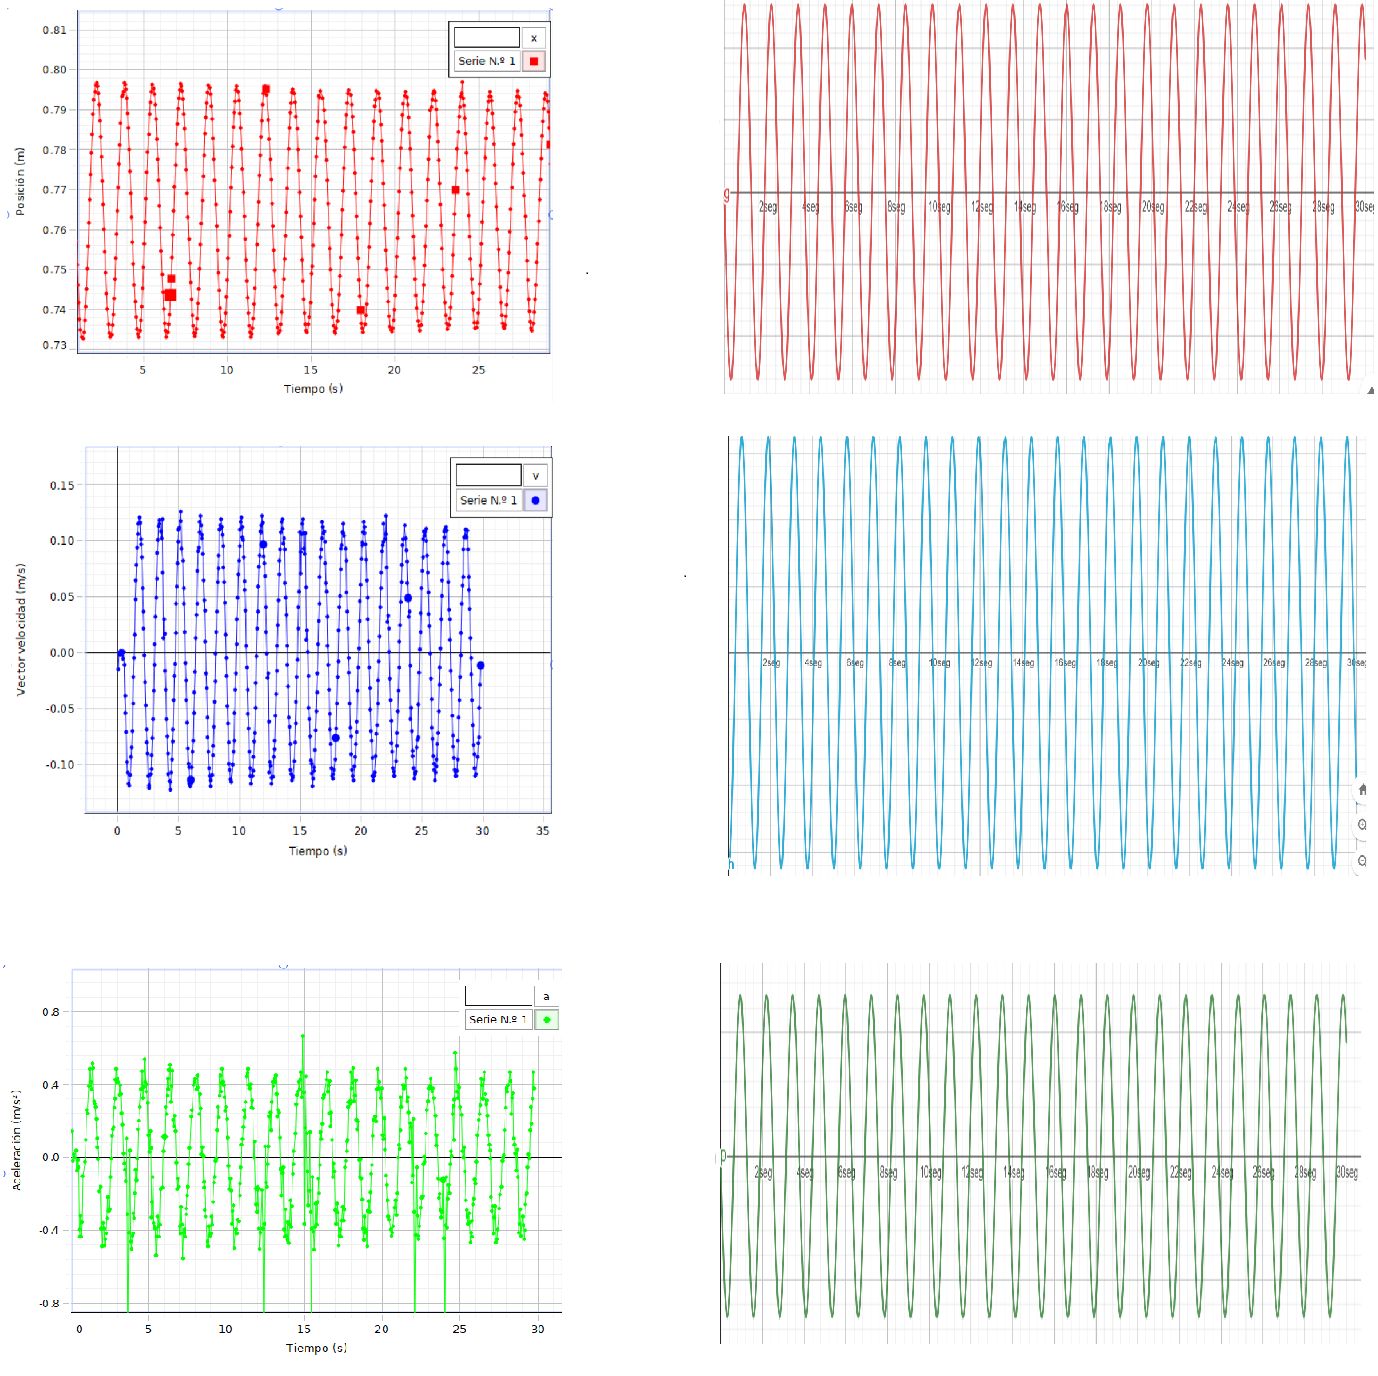
\includegraphics[width=1\linewidth]{h3cm.png}
    \caption{Graficas x/v/a vs t al compararse una por una con su grafica deducida analiticamente [3cm estiramiento]}
    \label{fig:enter-label}
\end{figure}\\

\begin{figure}[h]
    \centering
    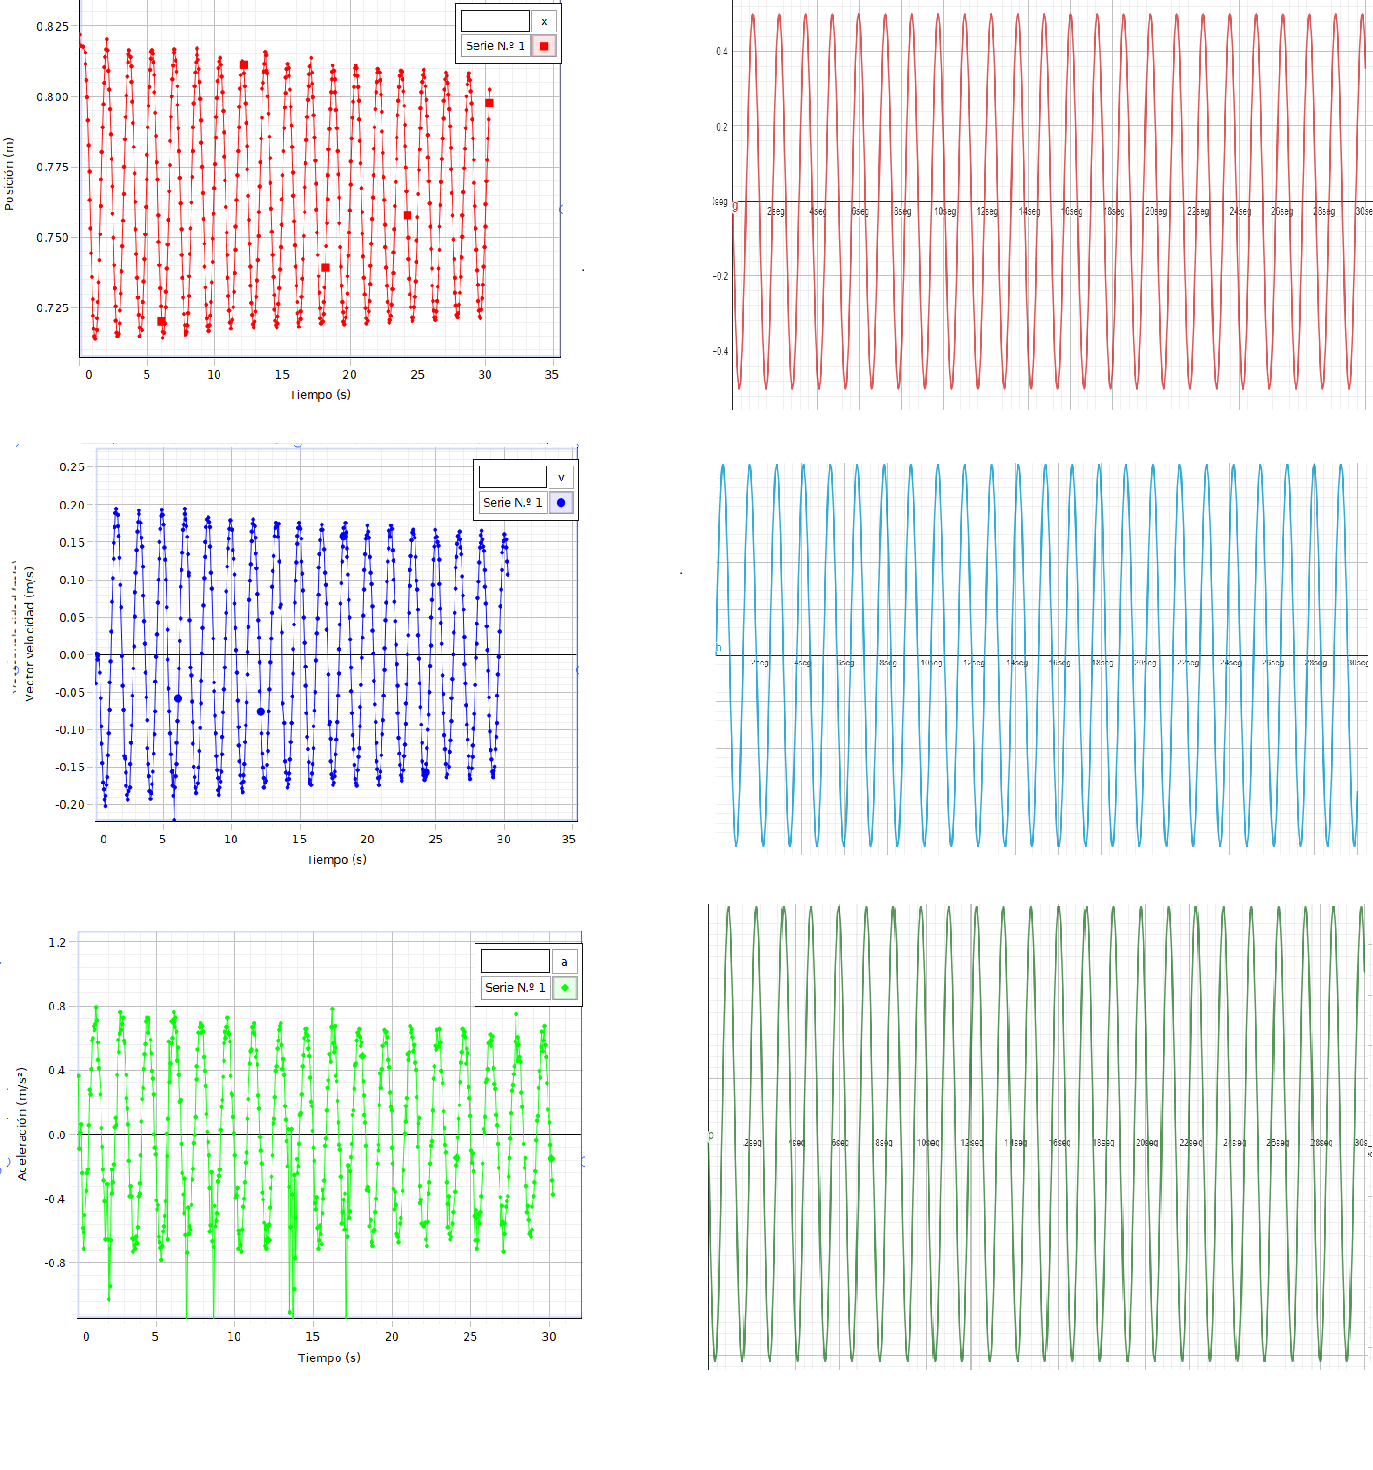
\includegraphics[width=1\linewidth]{h5cm.png}
    \caption{Graficas x/v/a vs t al compararse una por una con su grafica deducida analiticamente [5cm estiramiento]}
    \label{fig:enter-label}
\end{figure}\\
\newpage

\begin{figure}[h]
    \centering
    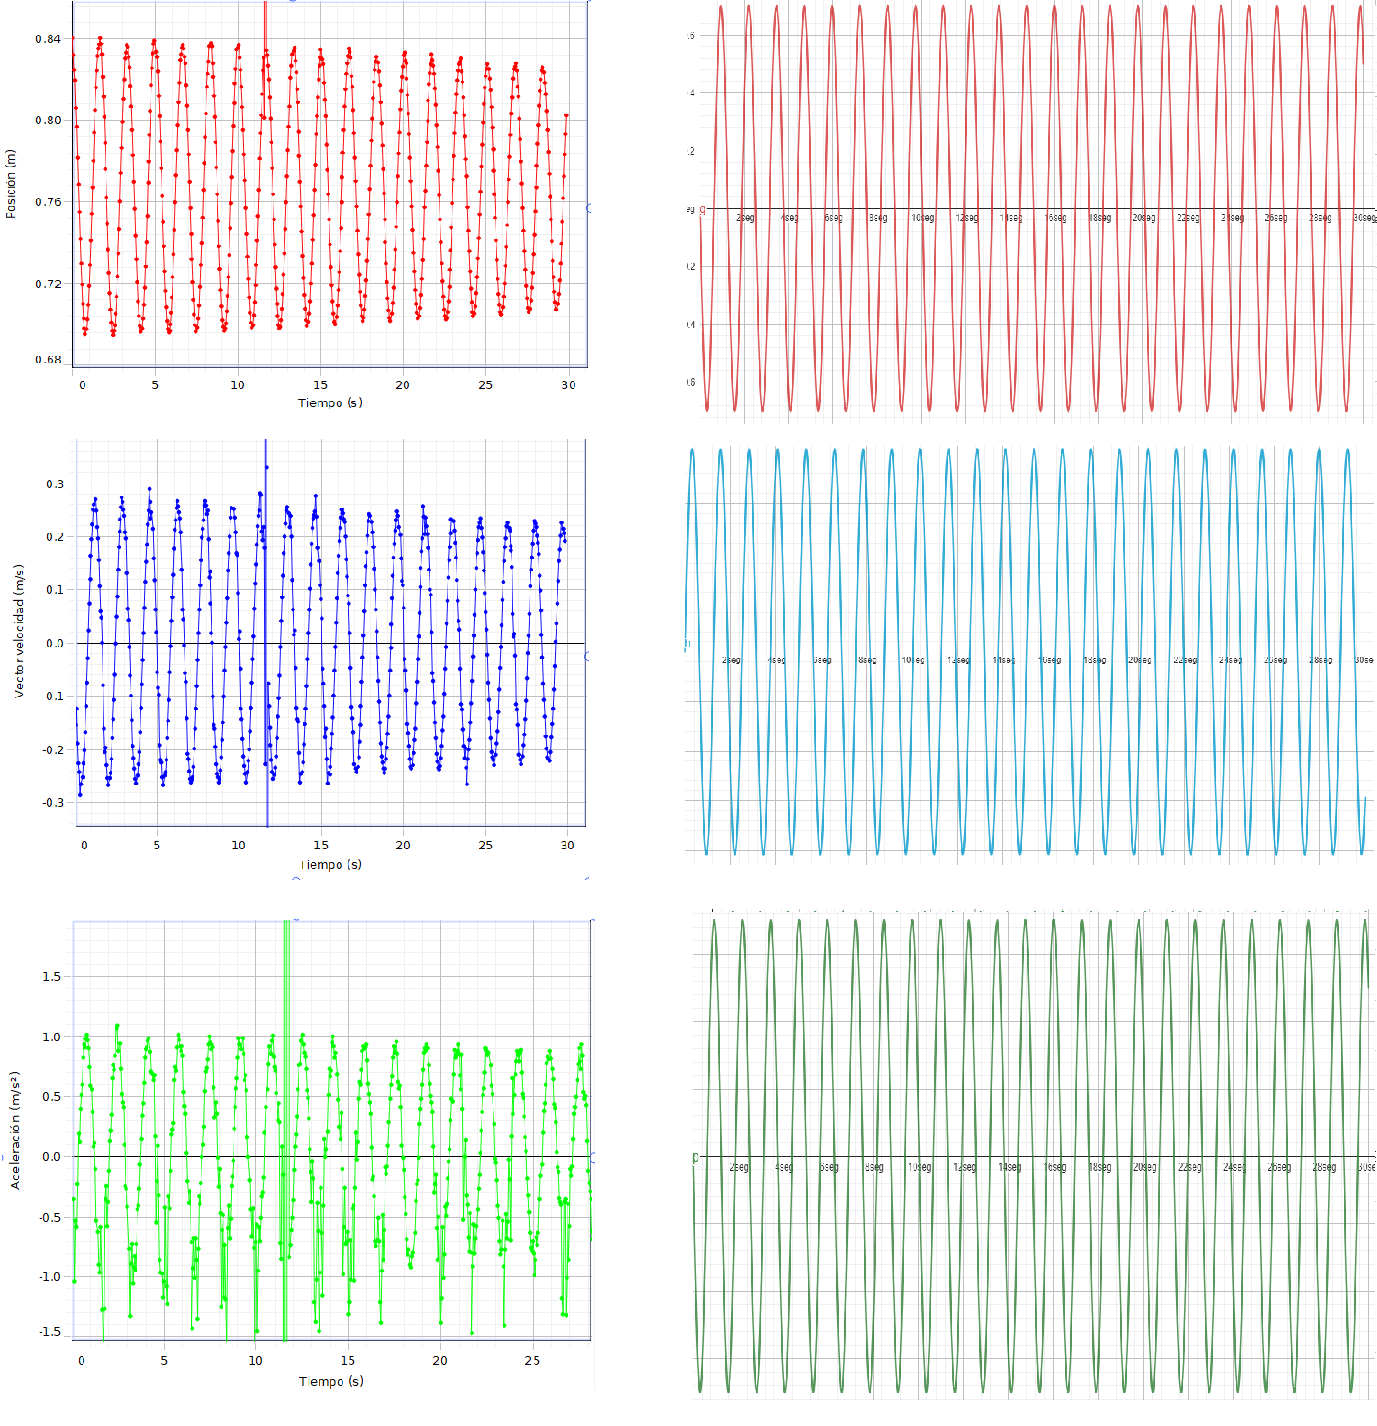
\includegraphics[width=1\linewidth]{h7cm.png}
    \caption{Graficas x/v/a vs t al compararse una por una con su grafica deducida analiticamente [7cm estiramiento]}
    \label{fig:enter-label}
\end{figure}\\
\newpage

\begin{figure}[h]
    \centering
    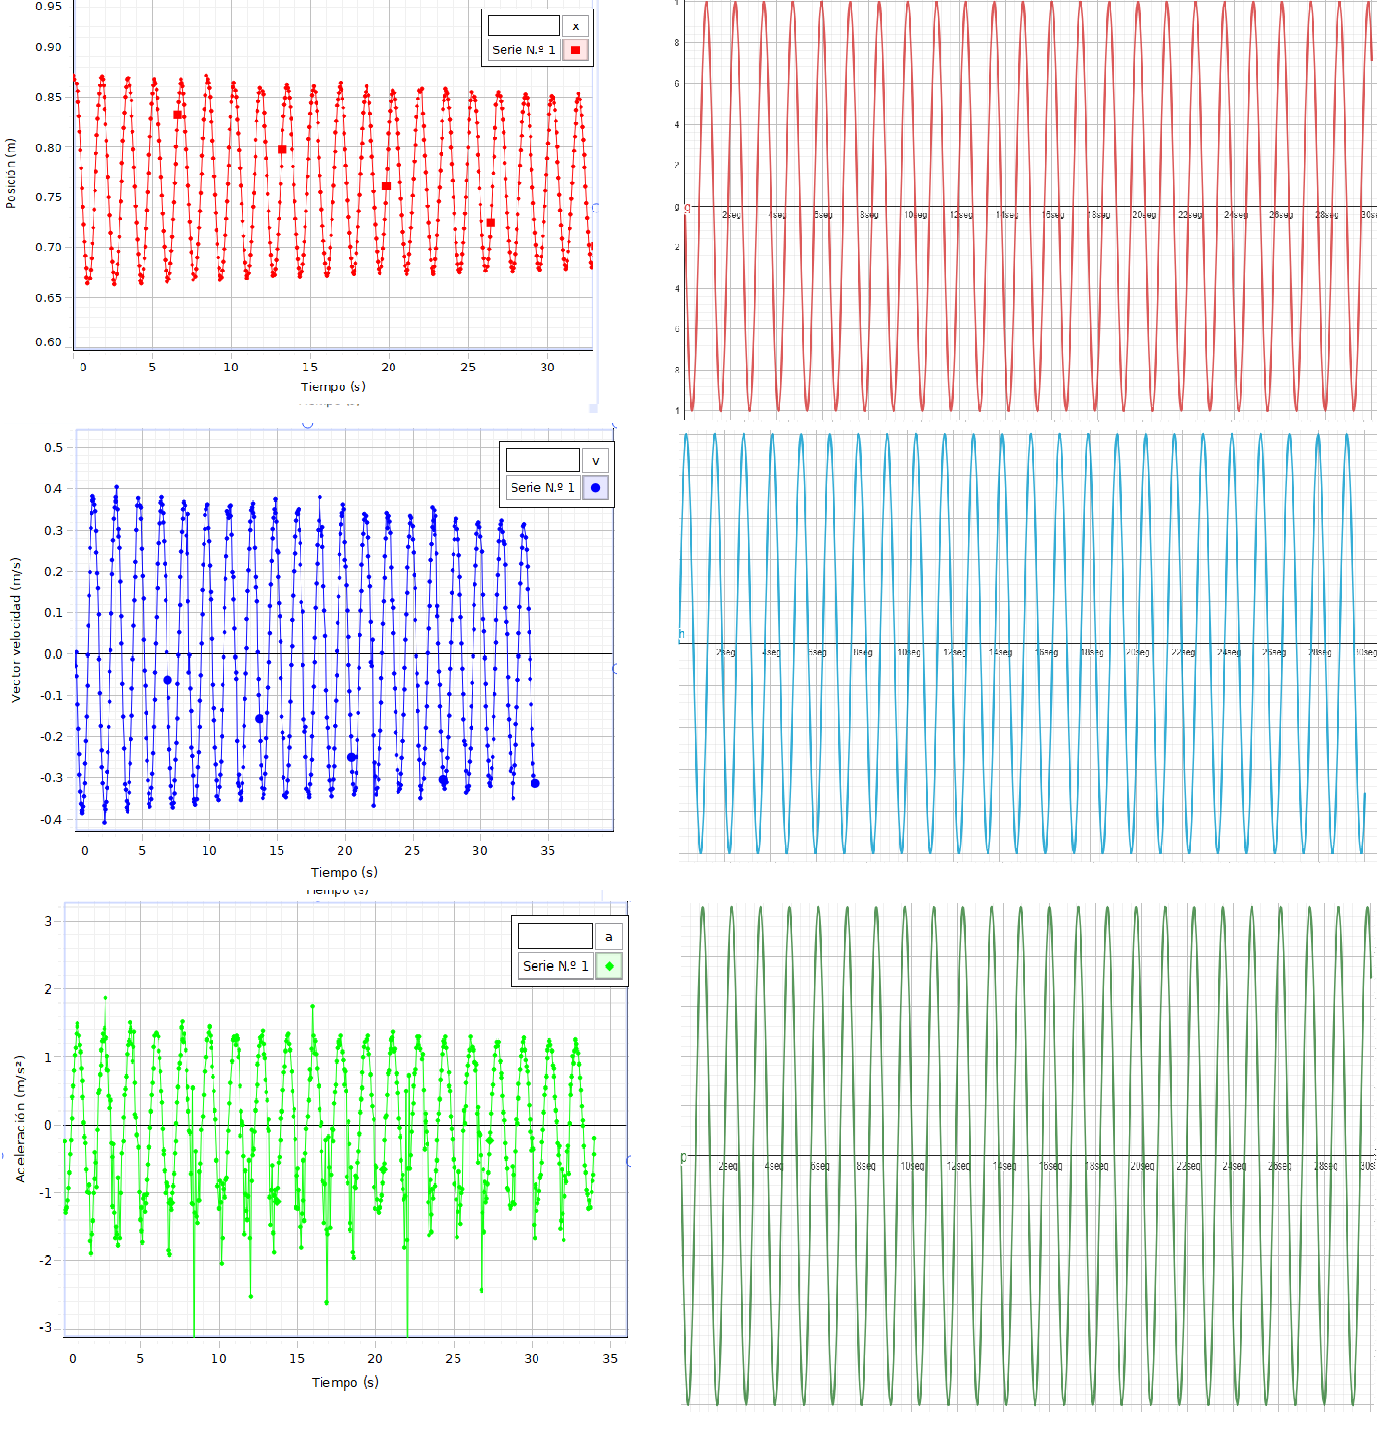
\includegraphics[width=1\linewidth]{h10cm.png}
    \caption{Graficas x/v/a vs t al compararse una por una con su grafica deducida analiticamente [10cm estiramiento]}
    \label{fig:enter-label}
\end{figure}\\
\newpage

\begin{figure}[h]
    \centering
    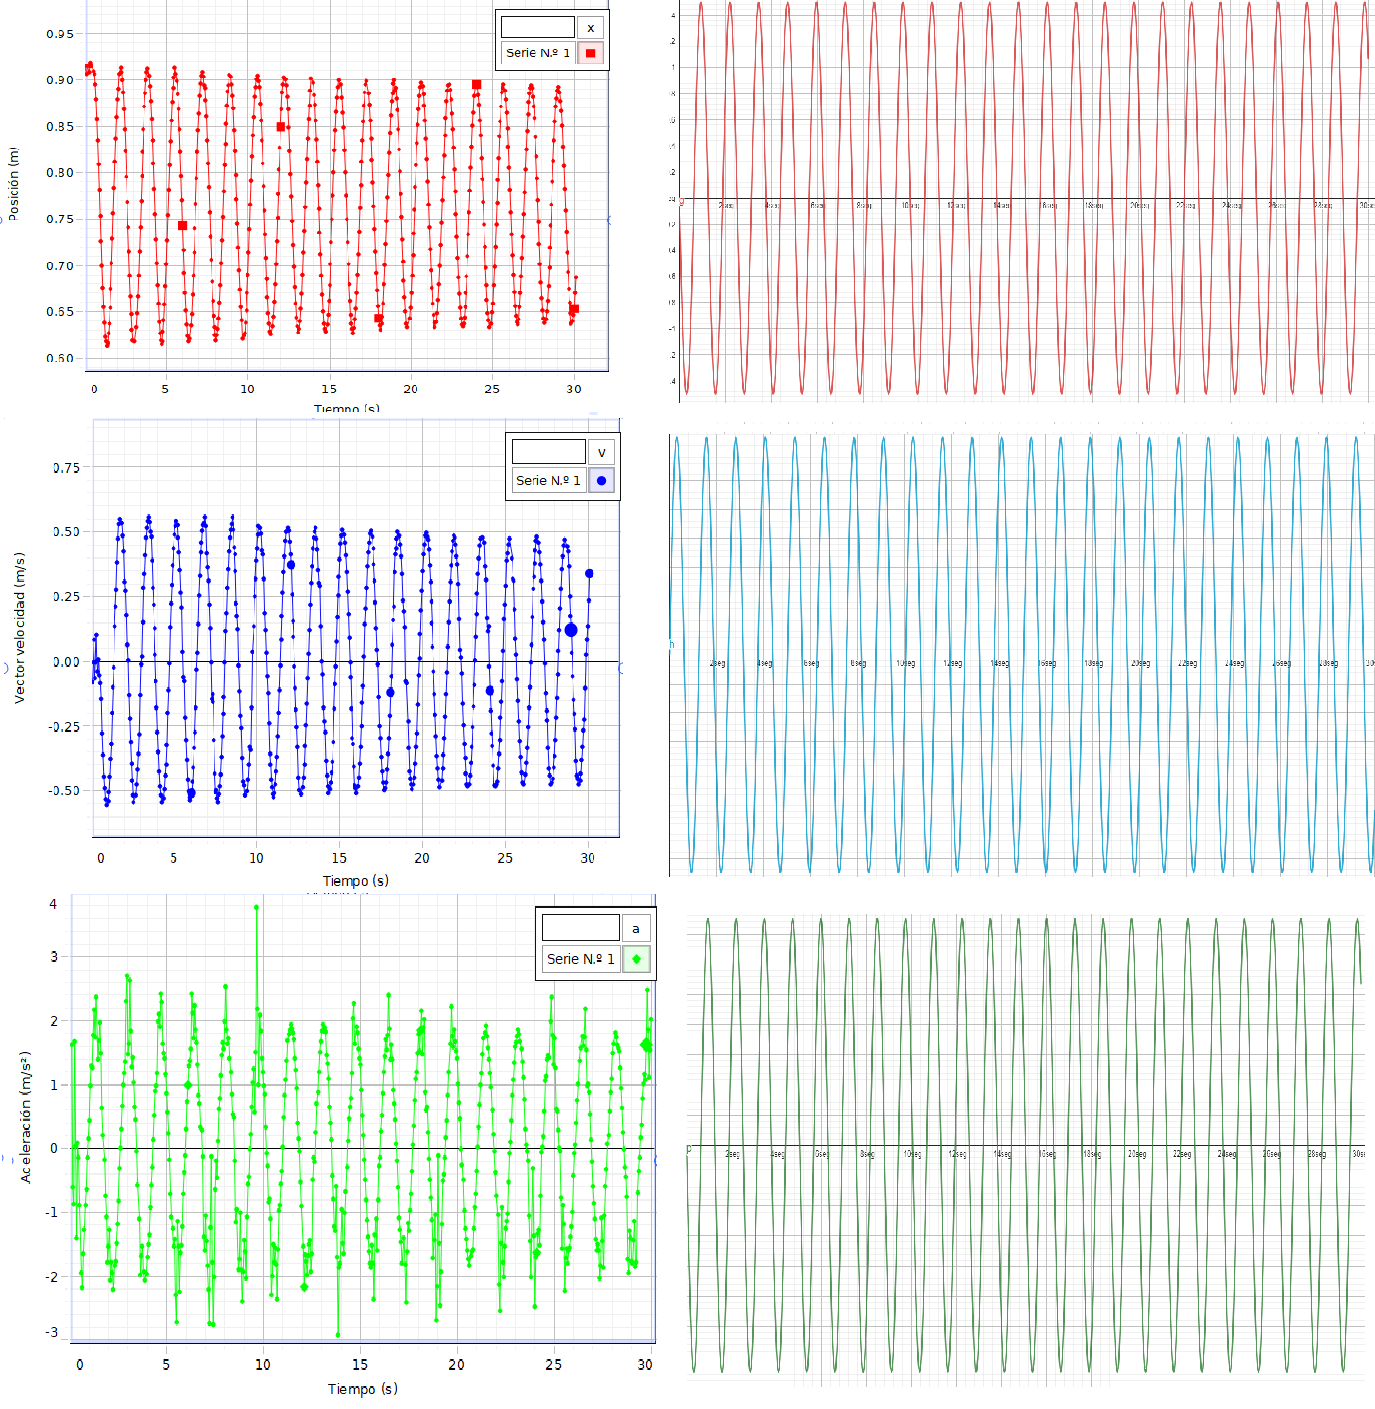
\includegraphics[width=1\linewidth]{h15cm.png}
    \caption{Graficas x/v/a vs t al compararse una por una con su grafica deducida analiticamente [15cm estiramiento]}
    \label{fig:enter-label}
\end{figure}\\
\newpage

\begin{figure}[h]
    \centering
    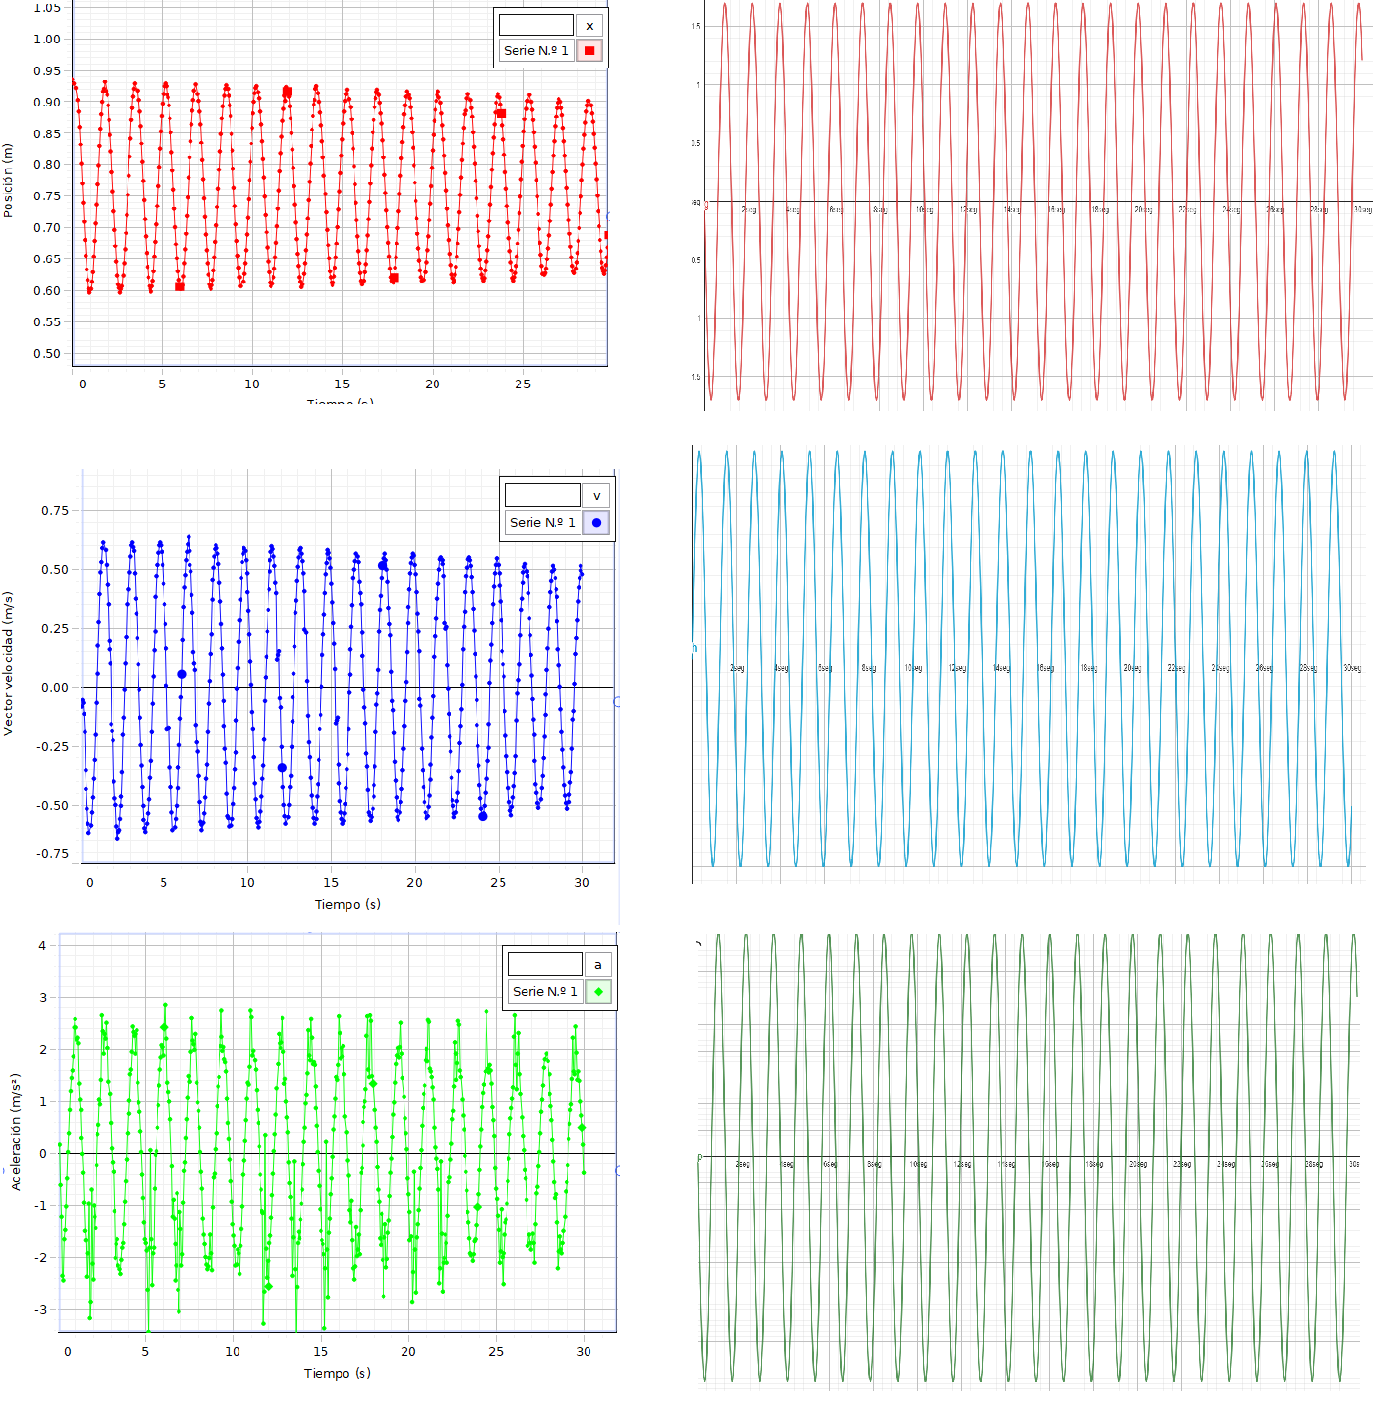
\includegraphics[width=1\linewidth]{h17cm.png}
    \caption{Graficas x/v/a vs t al compararse una por una con su grafica deducida analiticamente [17cm estiramiento]}
    \label{fig:enter-label}
\end{figure}\\
\newpage

\textit{ }
\begin{figure}[h]
    \centering
    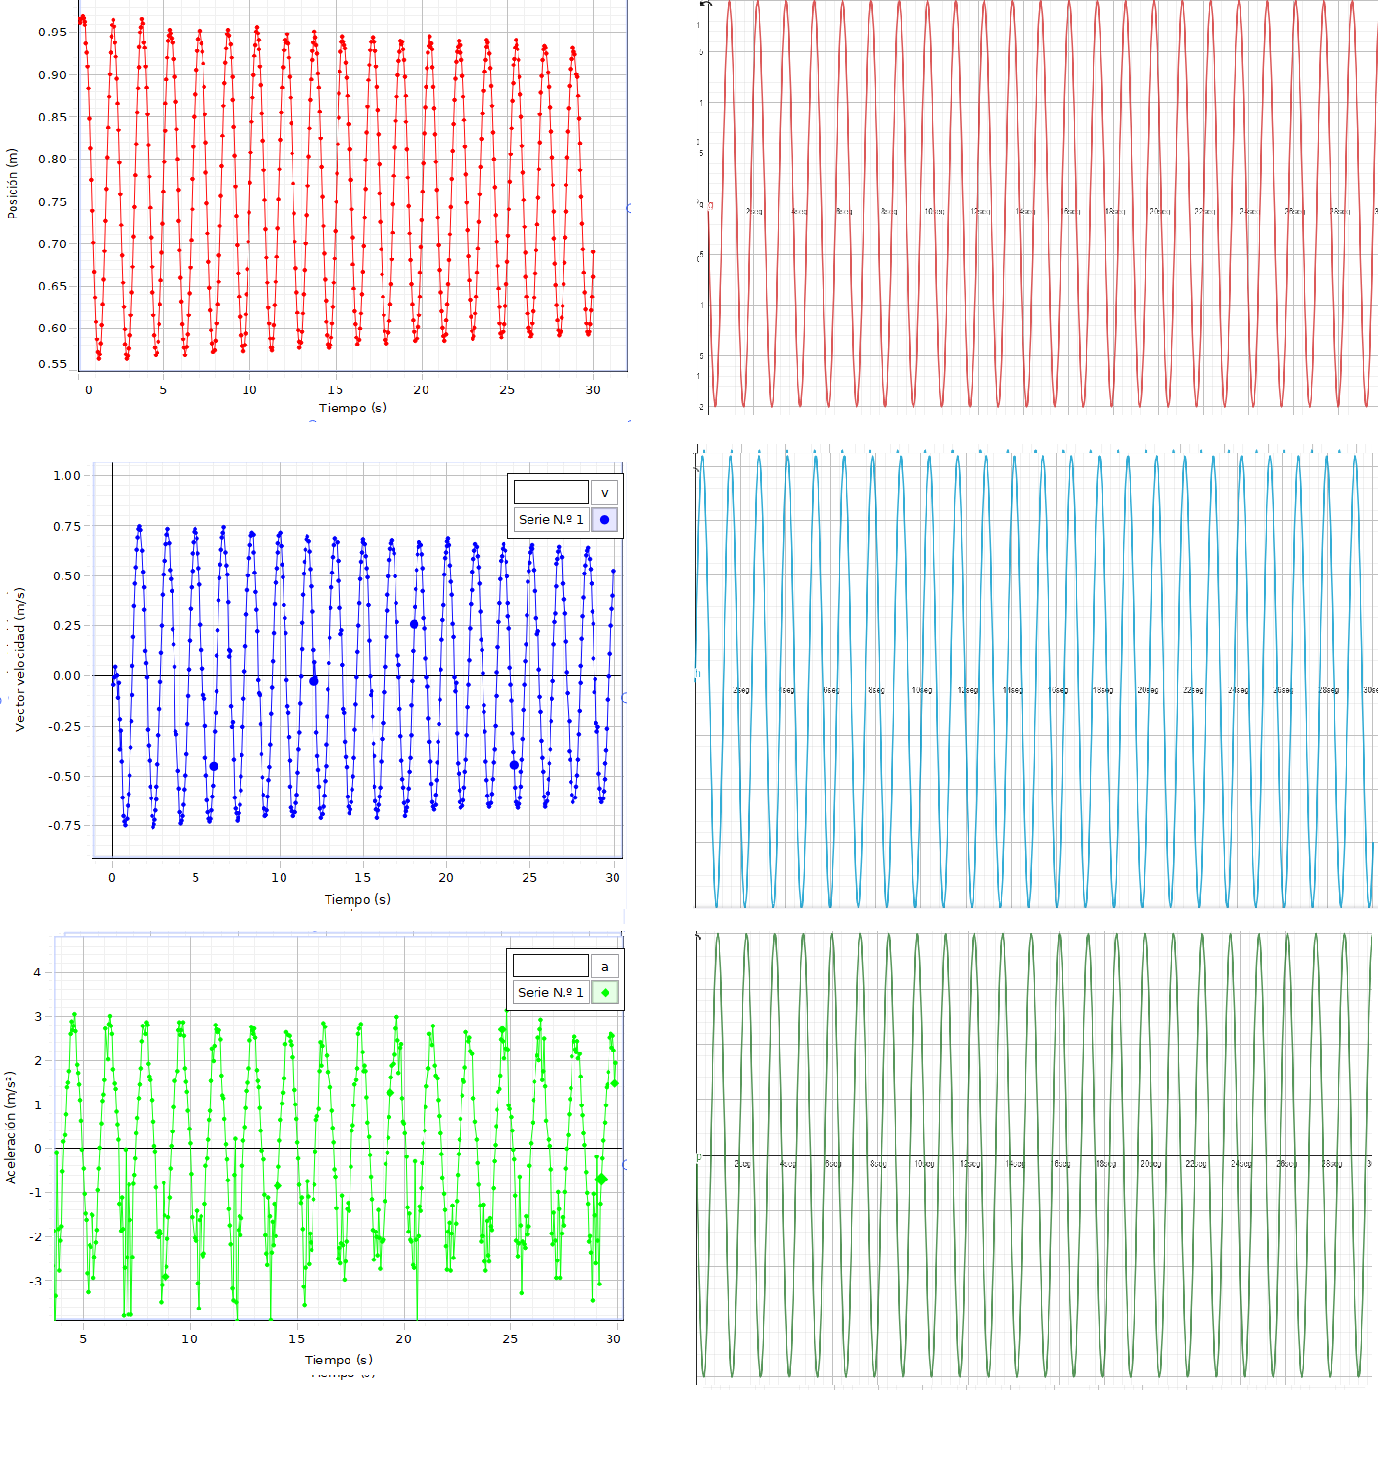
\includegraphics[width=1\linewidth]{h20cm.png}
    \caption{Graficas x/v/a vs t al compararse una por una con su grafica deducida analiticamente [20cm estiramiento]}
    \label{fig:enter-label}
\end{figure}\\
\newpage

\begin{figure}[h]
    \centering
    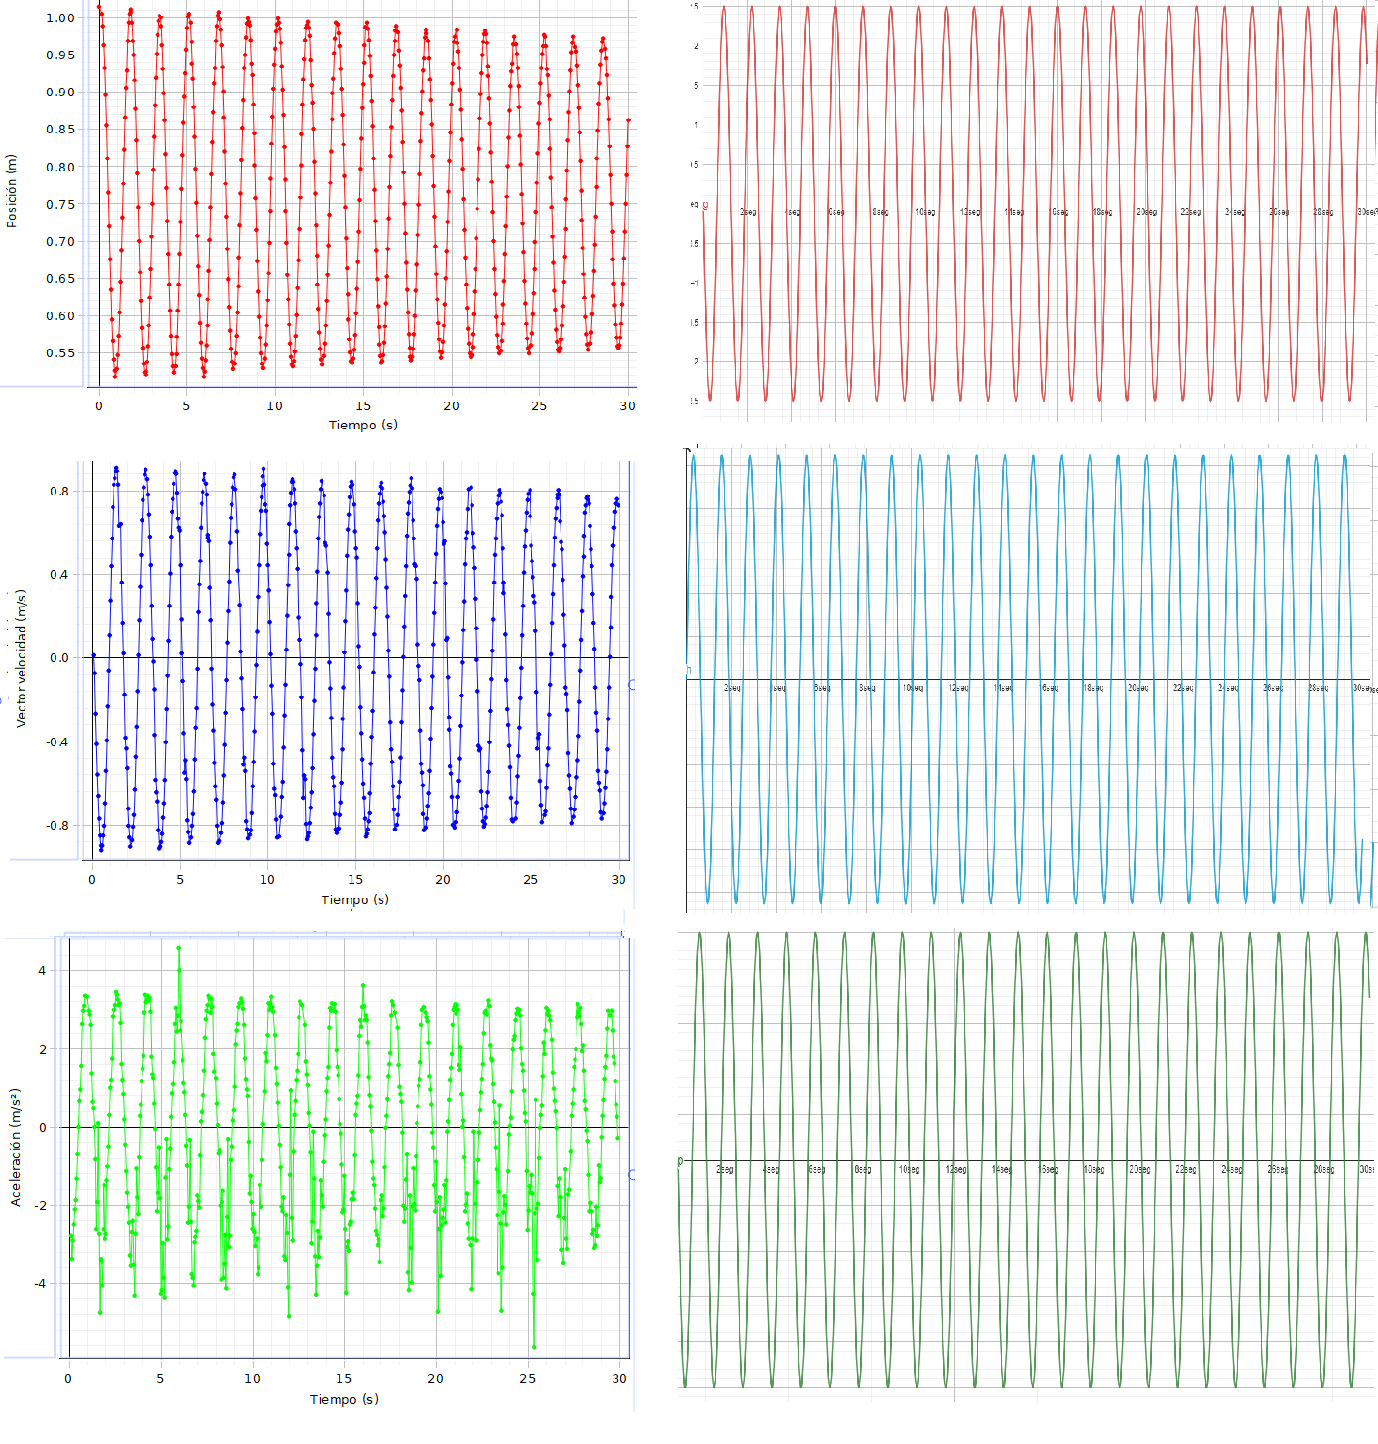
\includegraphics[width=1\linewidth]{h25cm.png}
    \caption{Graficas x/v/a vs t al compararse una por una con su grafica deducida analiticamente [25cm estiramiento]}
    \label{fig:enter-label}
\end{figure}\\
\newpage

\textit{ }
\begin{figure}[h]
    \centering
    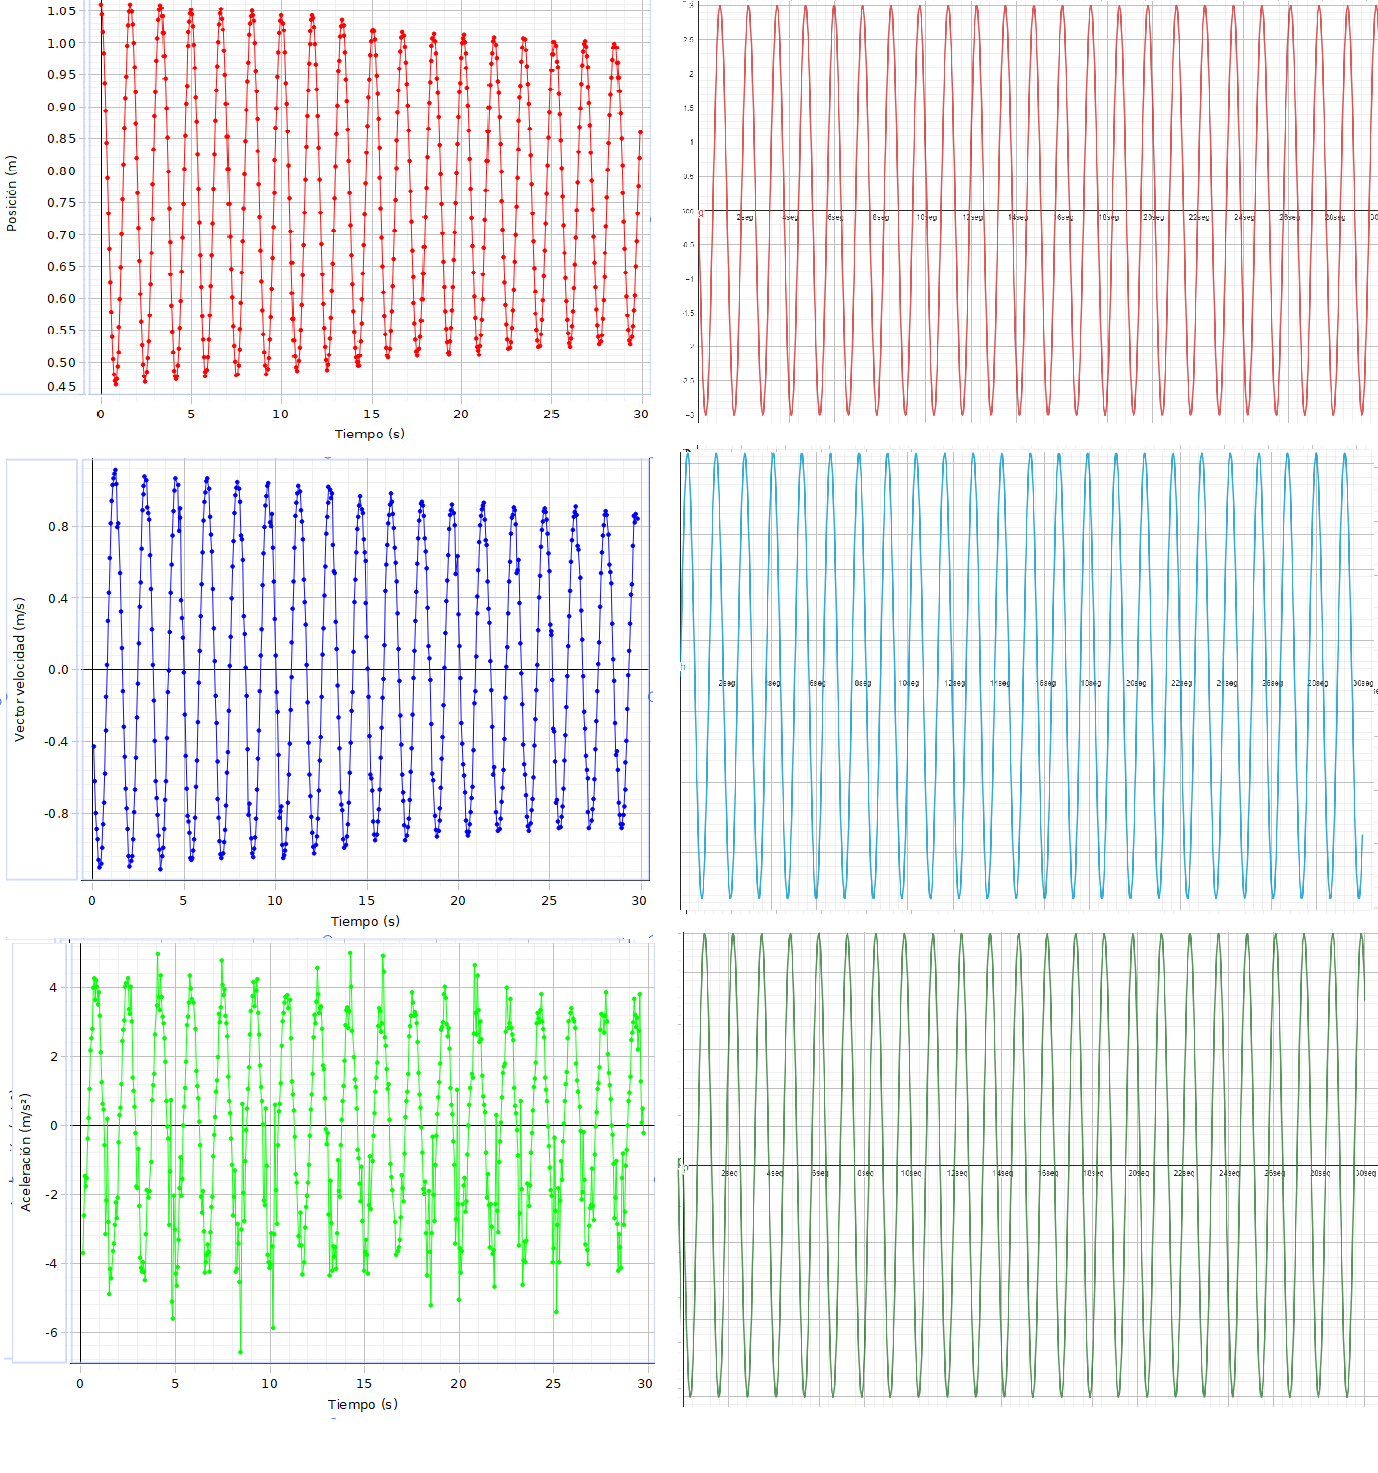
\includegraphics[width=1\linewidth]{h30cm.png}
    \caption{Graficas x/v/a vs t al compararse una por una con su grafica deducida analiticamente [30cm estiramiento]}
    \label{fig:enter-label}
\end{figure}\\
\newpage

\textit{ }
\begin{figure}[h]
    \centering
    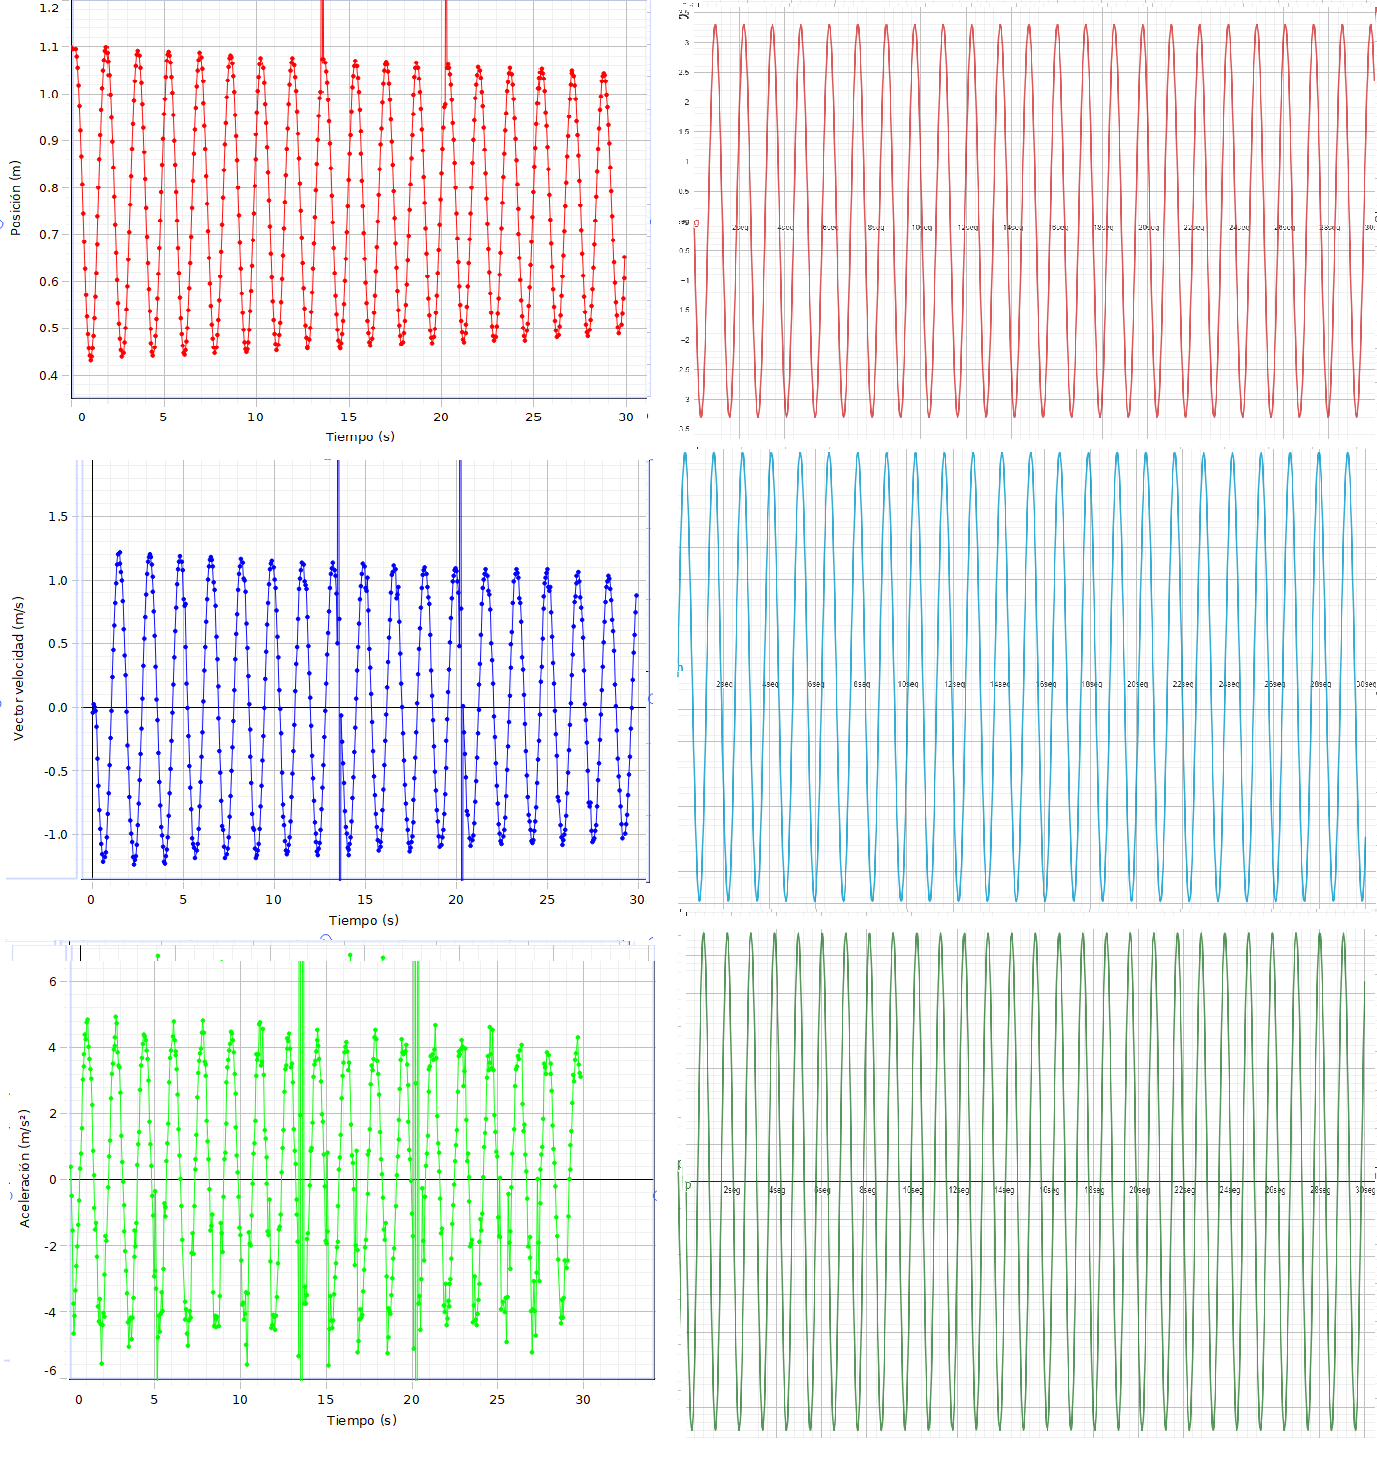
\includegraphics[width=1\linewidth]{h33cm.png}
    \caption{Graficas x/v/a vs t al compararse una por una con su grafica deducida analiticamente [33cm estiramiento]}
    \label{fig:enter-label}
\end{figure}\\
\newpage
\textit{ }
Nótese que las gráficas que yo he creado mejoran mucho con respecto a las del programa pues además de lo ya comentado usan el sistema [x]=dm, [v]=dm/s, [a]=dm/s pues así es totalmente legible con qué estamos tratando pues la gráfica que nos da el software además de estar desplazada en $y$ usa todas sus medidas en metros, que al ser datos muy pequeños es muy confuso. A continuación se adjuntará una comparación solo del último ángulo por la extrema dificultad en la interpretación de datos ya que se ha tomado una hora por cada gráfica en este tipo de movimiento amortiguado, por cuestiones de interacciones ambientales estas varían fuertemente en parámetros que no se pueden controlar en este laboratorio, en estas gráficas ahora variará el ángulo en lugar de la elongación, es por ello que mantendremos fijos 5cm, es importante resaltar que tenemos un conteo de 60 gráficas por cada ángulo así como tablas con cientos de valores con los cuales se han construído cada una de las gráficas, por lo que solo adjuntaremos las 3 mejores gráficas para cada ángulo con comparativa solo en el último ángulo quien físicamente debe presentar la mayor envolvente. \\

\begin{figure}[h]
    \centering
    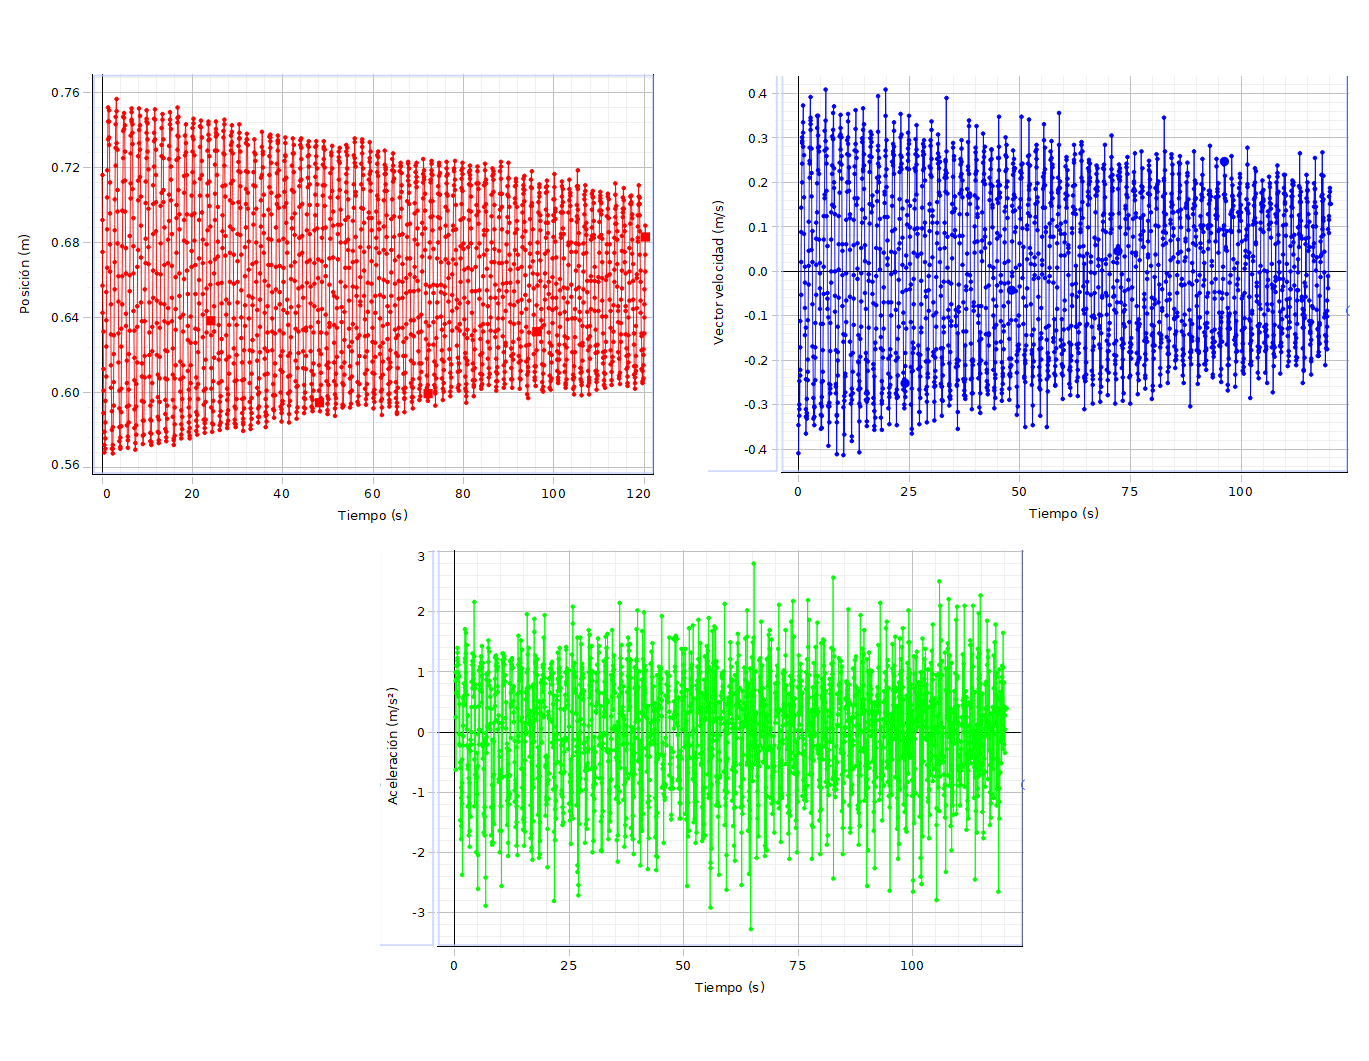
\includegraphics[width=0.85\linewidth]{4gi.png}
    \caption{Gráficas x/v/a vs t del movimiento armónico amortiguado [4 grados]}
    \label{fig:enter-label}
\end{figure}\\

\newpage
\begin{figure}[h]
    \centering
    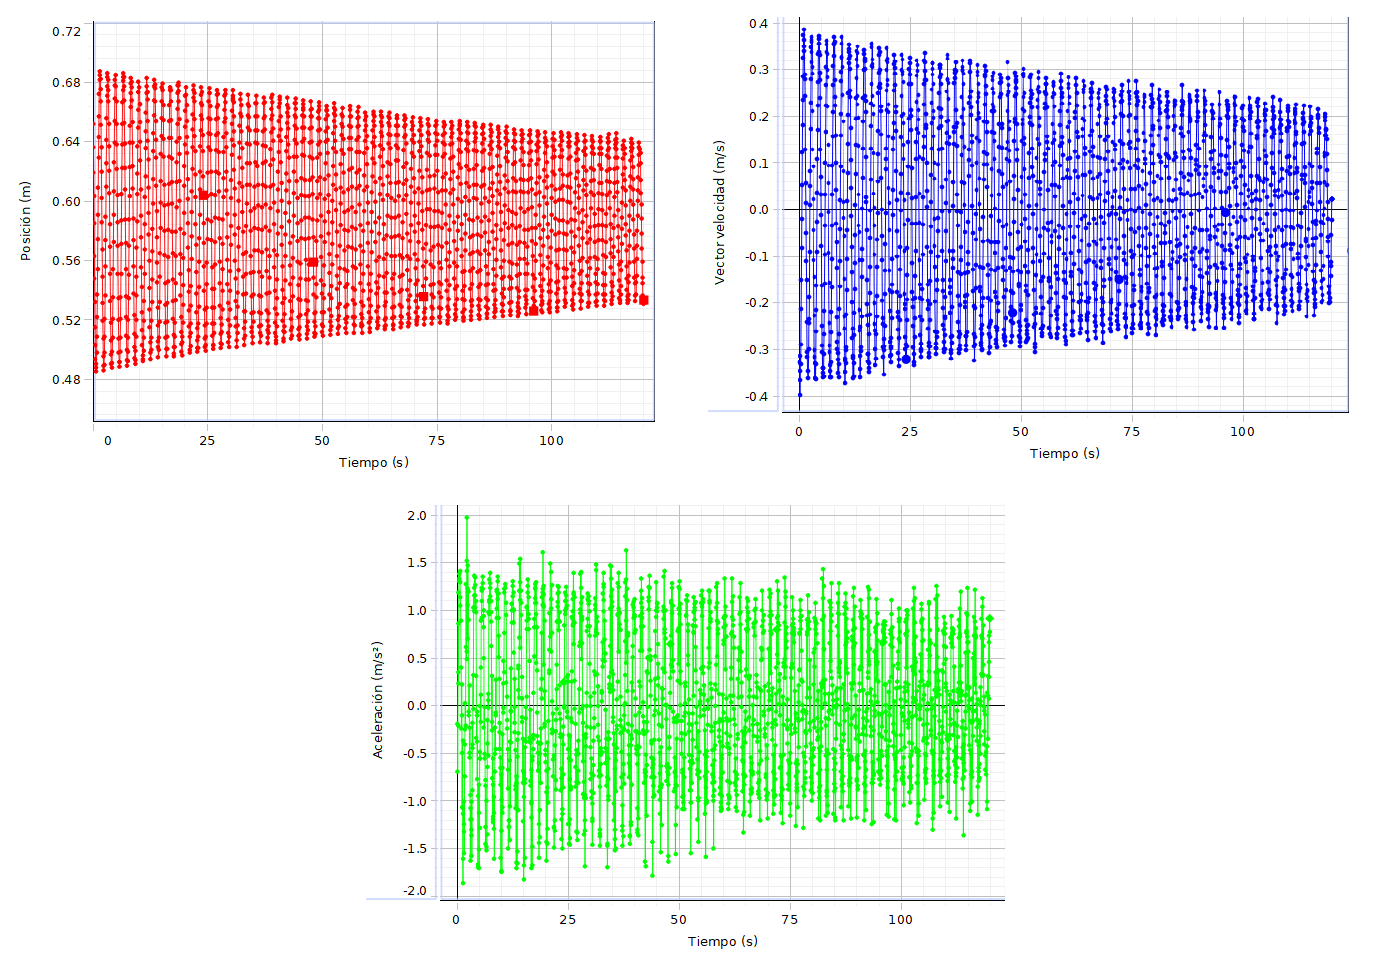
\includegraphics[width=0.7\linewidth]{8gi.png}
    \caption{Gráficas x/v/a vs t del movimiento armónico amortiguado [8 grados]}
    \label{fig:enter-label}
\end{figure}\\

\begin{figure}[h]
    \centering
    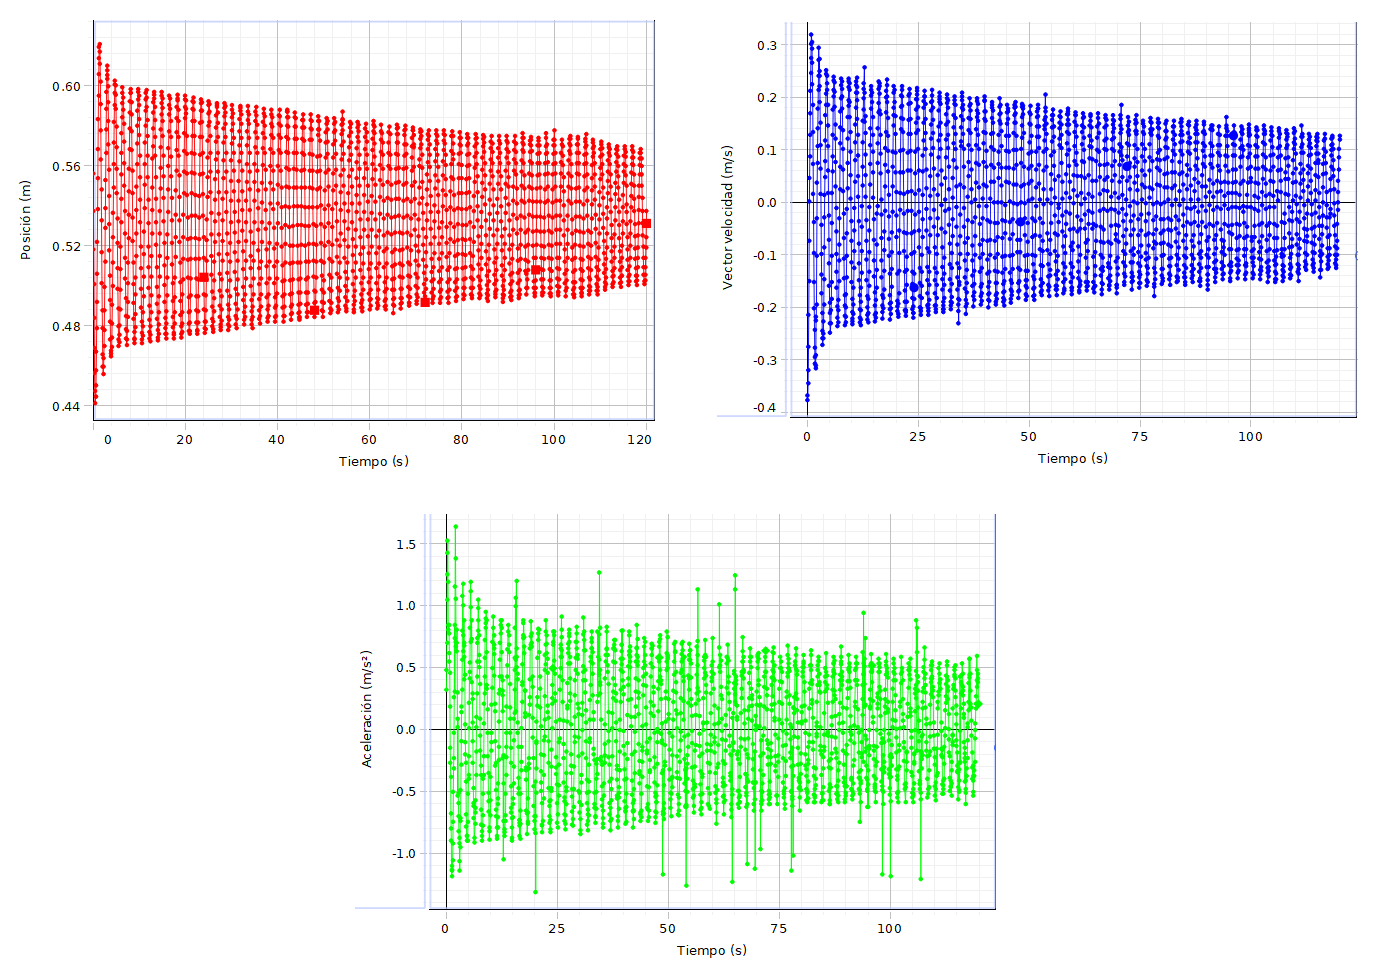
\includegraphics[width=0.7\linewidth]{12gi.png}
    \caption{Gráficas x/v/a vs t del movimiento armónico amortiguado [12 grados]}
    \label{fig:enter-label}
\end{figure}\\
\textit{   }
\newpage
\textit{   }

\begin{figure}[h]
    \centering
    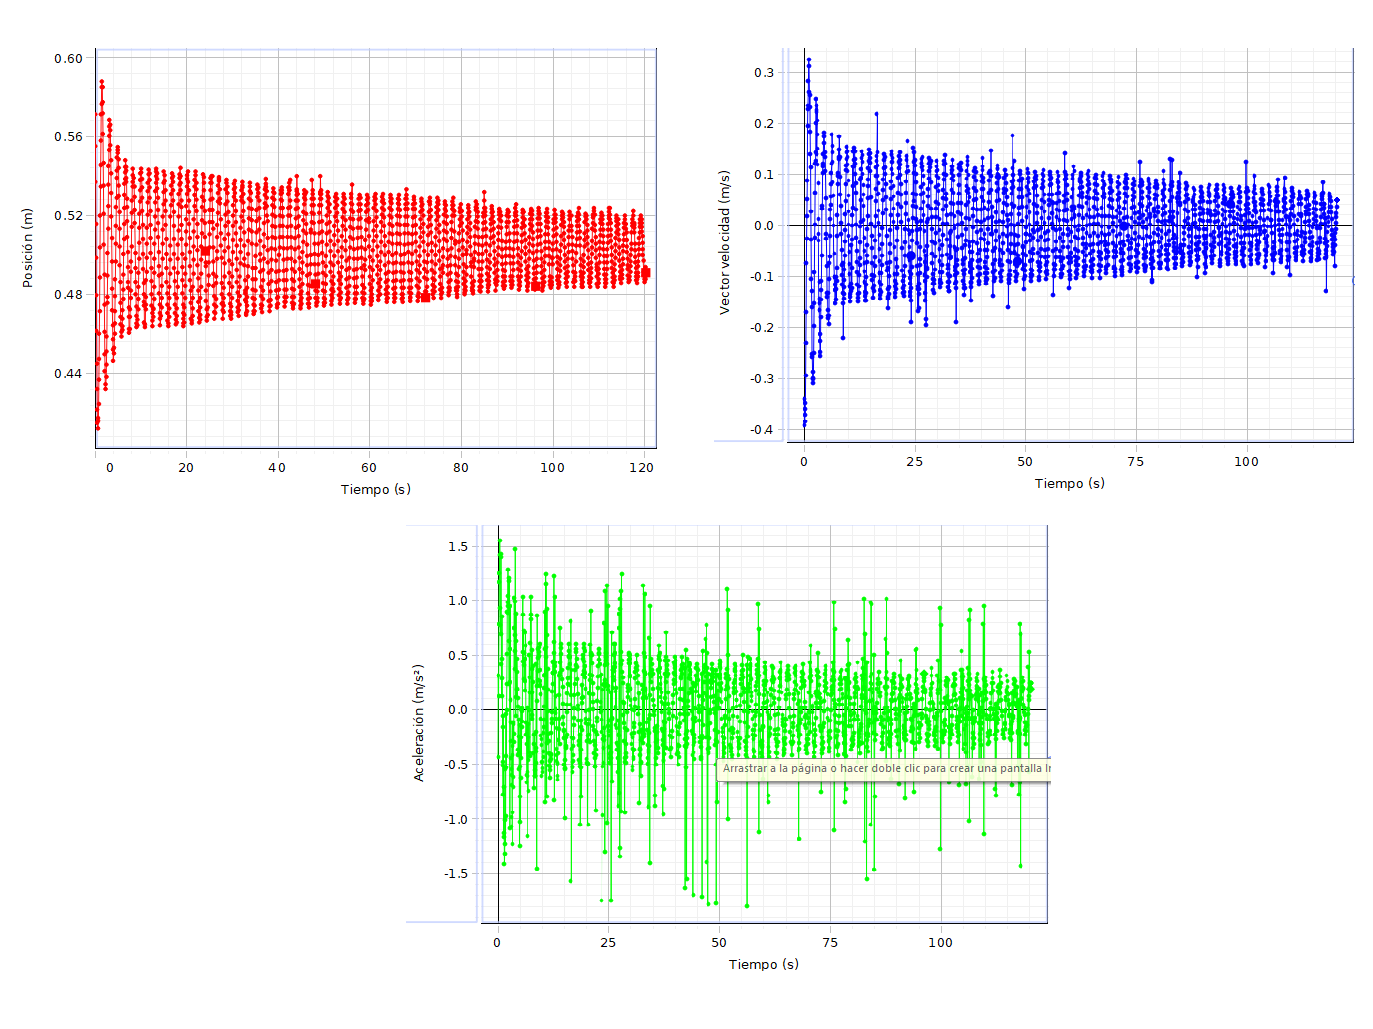
\includegraphics[width=0.85\linewidth]{16gi.png}
    \caption{Gráficas x/v/a vs t del movimiento armónico amortiguado [16 grados]}
    \label{fig:enter-label}
\end{figure}\\
\newpage

\begin{figure}[h]
    \centering
    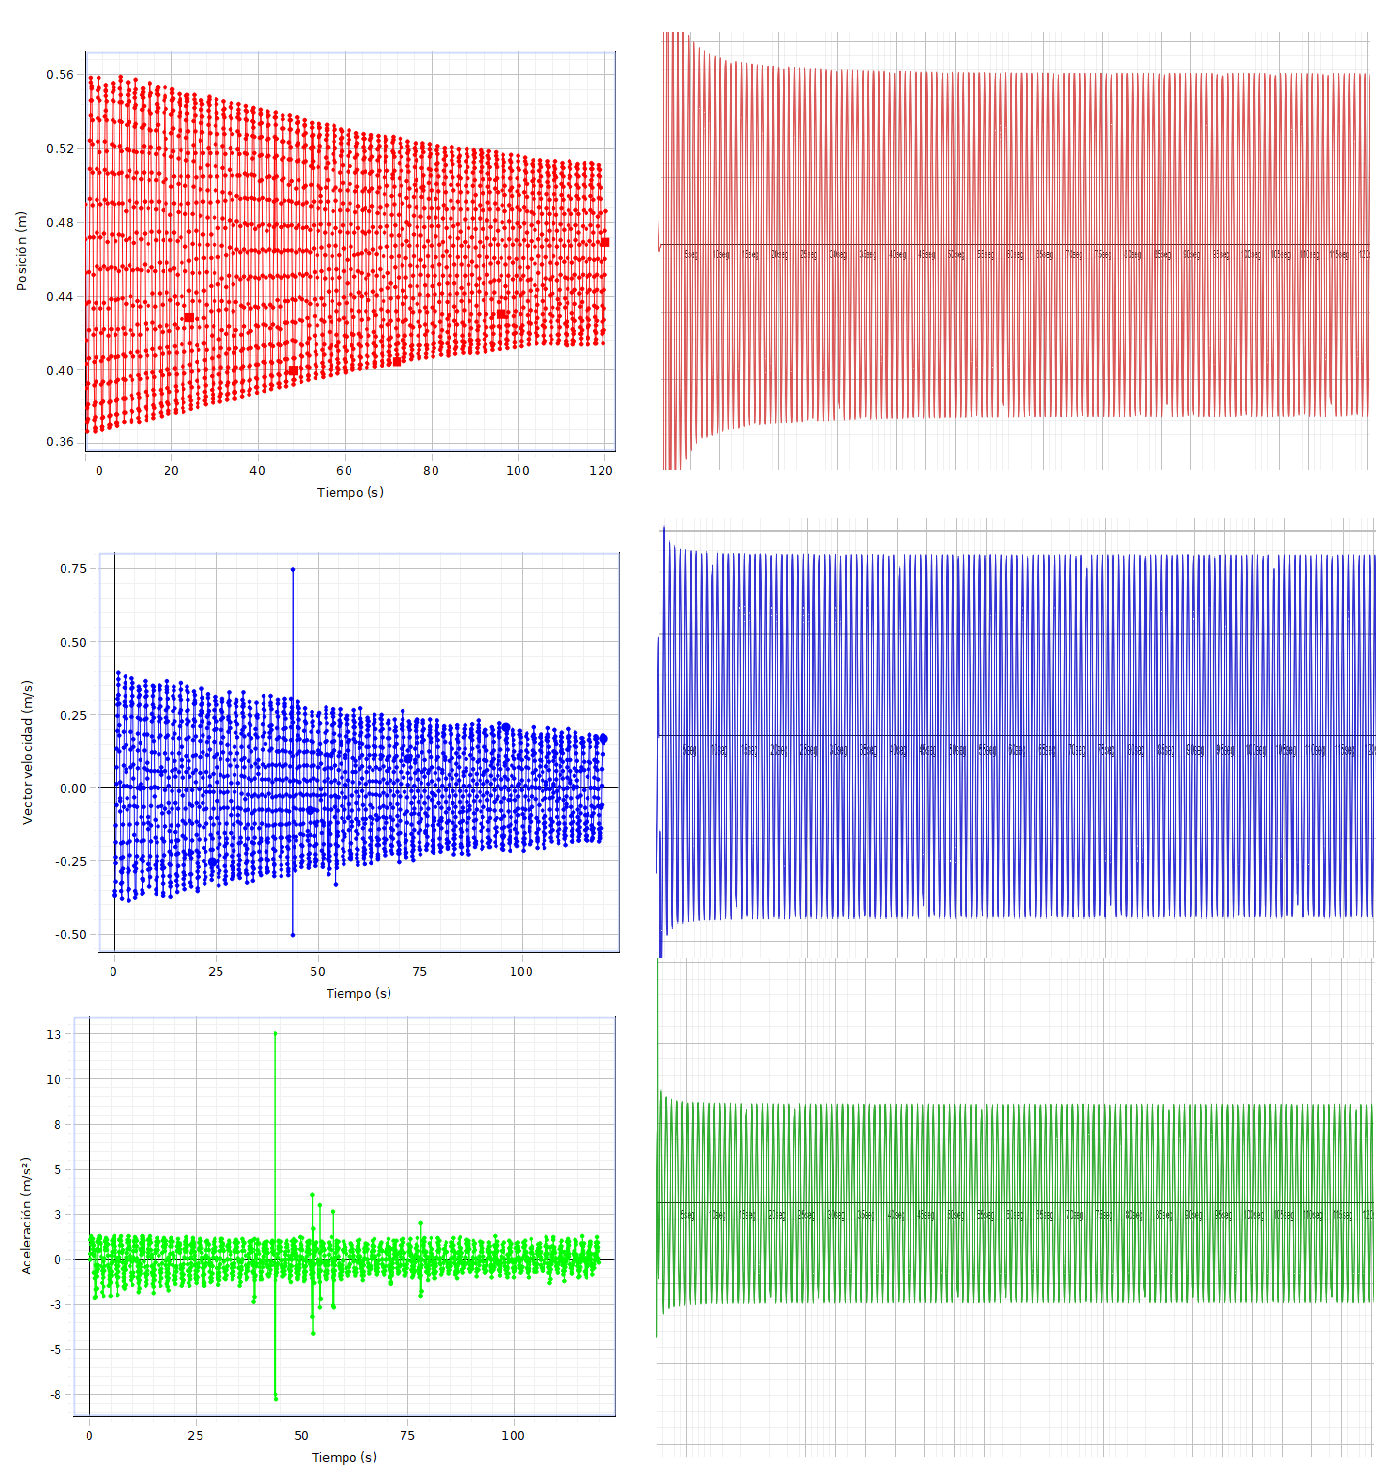
\includegraphics[width=1\linewidth]{20gi.png}
    \caption{Gráficas x/v/a vs t del movimiento armónico amortiguado [20 grados]}
    \label{fig:enter-label}
\end{figure}\\

\newpage
\section{Discusión de Resultados}
Para la primera parte del experimento, en la cual el riel de aire estaba en posición horizontal. Una vez que se le aplicaba una amplitud A al sistema y se sacaba al deslizador de su posición de equilibrio (en el que la fuerza neta que actuaba sobre el deslizador era 0), los resortes conectados a los extremos del deslizador comenzaban a ejercer una fuerza directamente proporcional a la amplitud inicial de elongación (fuerza de restitución); dichas fuerzas estaban ambas dirigidas en la misma dirección. 
\[ \Sigma F_{x} = -2K\Delta x\]
\[\Delta x = A\]
 Una vez el deslizador se desplaza debido a la elongación, por la cual adquiere una energía potencial elástica, cuando regresa al punto de equilibrio nuevamente, a pesar de que la fuerza neta que actúa sobre el deslizador es 0,tiene una energía cinética máxima, razón por la cual continúa desplazandose hacía el otro lado, y tiende a detenerse nuevamente en -A, pues las fuerzas que actúan son conservativas y se da la conversión bidireccional de energía potencial-cinética; si no hay fuerzas disipadoras en el sistema (como lo es la fricción), el sistema oscilará, sin cambiar su amplitud máxima, indefinidamente.
 Lo último es una consecuencia directa de la ley de la conservación de la energía. 
 \[E_{tot} = E_{Kmax};x=0\]
 \[U_{tot} = 2\left(\frac{1}{2}\right)Kx^{2} = Kx^{2} = E_{Kmax}\]
 \[K = \frac{E_{Kmax}}{x^{2}};x = A\]
 Para cada elongación distinta calculamos la constante de resorte: Obtuvimos 10 datos distintos que fluctuaban por muy poco; utilizamos la desviación estándar para calcular la inertidumbre asociada a los datos con los que calculamos la constante para cada elongación y, haciendo uso de derivadas parciales para la obtención de la incertidumbre indirecta, pues la magnitud calculada dependía de otras mediciones con incertidumbre, obtuvimos la incertidumbre asociada a la constante del resorte. Después calculamos el promedio de las constantes obtenidas.
 \[\Bar{K} = 2.917 \pm 0.138\frac{N}{m} \]
Aunque es físicamente imposible construir en la realidad un sistema que presente un movimiento oscilatorio sin que exista una perdida de energía, se pudo observar en las gráficas que para tiempos de medición cortos la amplitud máxima del sistema, mientras se daba la oscilación, se mantenía constante.
Por lo anteriormente mencionado, calcular la constante del resorte consta de igualar la energía cinética máxima (la velocidad instánea fue proporcionada por el sensor) a la energía potencial elástica máxima en la que x es A. Conocemos todos los datos, incluida la masa del deslizador, excepto k que se despeja para cada desplazamiento 

En la segunda parte, en la que el riel se inclina un ángulo, el tiempo de medición para cada amplitud fue mucho mayor al implementado en la primera parte; esto para que se apreciara la envolvente descrita en la gráfica de posición-tiempo. 
En las gráficas se puede ver que, con el paso del tiempo, la amplitud máxima para cada ciclo de oscilación disminuía paulatinamente y el periodo iba en aumento.
Los hechos mencionados previamente son características de un movimiento oscilatorio subamortiguado: la presencia de fuerzas disipadoras se vuelve aparente.
\[x = Ae^{-(b/2m)t}cos(\omega t + \theta)\]
b es una constante que describe la magnitud de la fuerza de amortiguamiento.

Lo anterior es contraintuitivo, pues si se realiza el análisis de fuerzas para un deslizador que se desplaza en una dirección a lo largo de un riel de aire inclinado, y el deslizador se encuentra conectado a un resorte de masa despreciable, podremos apreciar que las fuerzas que efectúan trabajo sobre el objeto son todas conservativas: la del resorte y la componte del peso del deslizador paralela al riel;  no existen fuerzas disipadoras, la energía mecánica del sistema se conserva, y la amplitud máxima para cada oscilación se mantiene constante.
\[\Sigma F = Wsin\varphi - 2Kx\]
Lo anterior nos recuerda que la física, teoricamente, no sólo se encarga de establecer leyes que describan la relación de hechos y fenómenos naturales, sino que también se encarga de efectuar una abstracción óptima de lo que observamos en el mundo físico. La propuesta de modelos simplificados hacen posible el estudio de la interacción entre la materia, a pesar de que estos no figuren en el mundo real, e incluso si se tratan de recrear en un ambiente controlado, como lo es un laboratorio, estén limitados.

\section{Conclusiones}
Se determinó la constante del resorte con precisión, y se pudo verificar la aplicabilidad del principio de conservación de la energía mecánica total en el sistema. El modelo de frenado \( F = -kx \) fue confirmado, y se determinó que el coeficiente \( k \) es proporcional a la masa del deslizador. La constante del resorte obtenida experimentalmente es de $\Bar{K} = 2.917 \pm 0.138\frac{N}{m}$\\

\newpage
\section{Apéndice de Ecuaciones Utilizadas}
\begin{itemize}
    \item Ley de Hooke: \( F = -kx \)
    \item Energía potencial elástica: \( U = \frac{1}{2}kx^2 \)
    \item Energía cinética: \( K = \frac{1}{2}mv^2 \)
    \item Conservación de la energía mecánica total: \( E_{\text{mec}} = U + K = \text{constante} \)
    \item Modelo de fuerza dependiente de la velocidad: \( F = -rv \)
\end{itemize} \\

\end{document}
